\documentclass[
  bibliography=totoc,     % Literatur im Inhaltsverzeichnis
  captions=tableheading,  % Tabellenüberschriften
  titlepage=firstiscover, % Titelseite ist Deckblatt (Finnd ich nicht so gut)
]{scrartcl}

% Paket float verbessern
\usepackage{scrhack}

% Warnung, falls nochmal kompiliert werden muss
\usepackage[aux]{rerunfilecheck}

% unverzichtbare Mathe-Befehle
\usepackage{amsmath}
% viele Mathe-Symbole
\usepackage{amssymb}
% Erweiterungen für amsmath
\usepackage{mathtools}

%\usepackage{physics}

% Fonteinstellungen
\usepackage{fontspec}
% Latin Modern Fonts werden automatisch geladen
% Alternativ zum Beispiel:
%\setromanfont{Libertinus Serif}
%\setsansfont{Libertinus Sans}
%\setmonofont{Libertinus Mono}

% Wenn man andere Schriftarten gesetzt hat,
% sollte man das Seiten-Layout neu berechnen lassen
\recalctypearea{}

% deutsche Spracheinstellungen
\usepackage[ngerman]{babel}


\usepackage[
  math-style=ISO,    % ┐
  bold-style=ISO,    % │
  sans-style=italic, % │ ISO-Standard folgen
  nabla=upright,     % │
  partial=upright,   % ┘
  warnings-off={           % ┐
    mathtools-colon,       % │ unnötige Warnungen ausschalten
    mathtools-overbracket, % │
  },                       % ┘
]{unicode-math}

% traditionelle Fonts für Mathematik
\setmathfont{Latin Modern Math}
% Alternativ zum Beispiel:
%\setmathfont{Libertinus Math}

\setmathfont{XITS Math}[range={scr, bfscr}]
\setmathfont{XITS Math}[range={cal, bfcal}, StylisticSet=1]

% Zahlen und Einheiten
\usepackage[
  locale=DE,                   % deutsche Einstellungen
  separate-uncertainty=true,   % immer Unsicherheit mit \pm
  per-mode=symbol-or-fraction, % / in inline math, fraction in display math
]{siunitx}

% chemische Formeln
\usepackage[
  version=4,
  math-greek=default, % ┐ mit unicode-math zusammenarbeiten
  text-greek=default, % ┘
]{mhchem}

% richtige Anführungszeichen
\usepackage[autostyle]{csquotes}

% schöne Brüche im Text
\usepackage{xfrac}

% Standardplatzierung für Floats einstellen
\usepackage{float}
\floatplacement{figure}{htbp}
\floatplacement{table}{htbp}

% Floats innerhalb einer Section halten
\usepackage[
  section, % Floats innerhalb der Section halten
  below,   % unterhalb der Section aber auf der selben Seite ist ok
]{placeins}

% Seite drehen für breite Tabellen: landscape Umgebung
\usepackage{pdflscape}

% Captions schöner machen.
\usepackage[
  labelfont=bf,        % Tabelle x: Abbildung y: ist jetzt fett
  font=small,          % Schrift etwas kleiner als Dokument
  width=0.9\textwidth, % maximale Breite einer Caption schmaler
]{caption}
% subfigure, subtable, subref
\usepackage{subcaption}

% Grafiken können eingebunden werden
\usepackage{graphicx}
\usepackage{wrapfig}

% schöne Tabellen
\usepackage{booktabs}

% Verbesserungen am Schriftbild
\usepackage{microtype}

% Literaturverzeichnis
\usepackage[
  backend=biber,
  sorting=none
]{biblatex}
% Quellendatenbank
\addbibresource{lit.bib}
\addbibresource{programme.bib}

% Hyperlinks im Dokument
\usepackage[
  german,
  unicode,        % Unicode in PDF-Attributen erlauben
  pdfusetitle,    % Titel, Autoren und Datum als PDF-Attribute
  pdfcreator={},  % ┐ PDF-Attribute säubern
  pdfproducer={}, % ┘
]{hyperref}
% erweiterte Bookmarks im PDF
\usepackage{bookmark}

% Trennung von Wörtern mit Strichen
\usepackage[shortcuts]{extdash}

%\setcounter{tocdepth}{3} % + subsubsections



\author{%
  Clara Sondermann \\%
  \href{mailto:clara.sondermann@tu-dortmund.de}{clara.sondermann@tu-dortmund.de}%
  \and%
  Enno Wellmann \\%
  \href{mailto:enno.wellmann@tu-dortmund.de}{enno.wellmann@tu-dortmund.de}%
}
\publishers{TU Dortmund – Fakultät Physik}


\newcommand*\diff{\mathop{}\!\mathrm{d}}

\NewDocumentCommand \OverfullCenter {+m} {
\noindent\makebox[\linewidth]{#1} }

\usepackage{adjustbox}

\newcommand*\diff{\mathop{}\!\mathrm{d}}

\NewDocumentCommand \OverfullCenter {+m} {
\noindent\makebox[\linewidth]{#1} }

\title{V308: Spulen und Magnetfelder}
\date{Durchführung: 13.12.2022, Abgabe: 20.12.2022}


\begin{document}
\maketitle

\thispagestyle{empty} 
\tableofcontents
\newpage
\setcounter{page}{1}

\input{Inhalte/A_Ziel_Theroie_Durchführung.tex}
    
\section{Auswertung}

\subsection{Hysteresekurve}
In diesem Versuch wird die Magnetisierung eines Eisenkerns betrachtet.
Wie in Abschnitt \ref{sec:A_Hysterese_Drcf} beschrieben wird der Strom nach und nach variiert 
und den Magnetfeldern gegenübergestellt.
Wie in \ref{eq:vereinfachungsgleichung} dargestellt ist die Magnetisierung des eisenkerns nahezu äquivalent zu dem tatsächlich messbaren Magnetfeld.
Das äußere Magnetfeld berechnet sich wie in Gleichung \ref{eq:toroid} mit
\begin{align}
    H = \frac{B}{\mu}
    H = \frac{n}{2 \pi r_\text{T}}. I
\end{align}
Bei der gegebenen Toroidspule beträgt der Radius $r_\text{T}= \qty{13.5}{cm}$ und die Windungszahl $n = 595$
Da $H$ proportional zu $I$ ist wird das Magnetfeld in Tabelle \ref{tab:hysterese_werte}
und in \ref{fig:Hysteresekurve_werte} gegen die Stromstärke aufgestellt.



%Für die Hysteresekurve wird allerdings die Magnetfeldstärke im Vakuum $H$ gebraucht.
%Diese berechnet sich wie in Gleichung \ref{eq:toroid} mit
%\begin{align*}
%    H = \frac{B}{\mu_0}
%    H =  \frac{1}{\mu_0} \frac{n}{2 \pi r_\text{T}} I
%\end{align*}
%Bei der gegebenen Toroidspule beträgt der Radius $r_\text{T}= \qty{13.5}{cm}$ und die Windungszahl $n = 595$
%Das Magnetische Moment berechnet sich analog zu Gleichung \ref{eq:Magnetisierung}
%\begin{align*}
%    M = \frac{B}{\mu_0} - H
%\end{align*}


%%% Tabelle mit Werten


\begin{table}
    \centering
    
    \OverfullCenter{
    \begin{tabular}{
        S[table-format=1.1]
        S[table-format=3.1]
        S[table-format=4.1]
        S[table-format=1.1]
        S[table-format=3.1]
        S[table-format=4.1]
        S[table-format=1.1]
        S[table-format=3.1]
        S[table-format=4.1]
    }
    \toprule
    \multicolumn{3}{c}{Neukruve} &
    \multicolumn{3}{c}{Absinkende Stromstärke} &
    \multicolumn{3}{c}{Steigende Stromstärke} \\
    {$I/ \unit{\ampere}$} & {$B\simeq \mu_0 M/ \unit{\milli\tesla}$} & {$H / (\unit{\ampere \per \meter})$} &   
    {$I/ \unit{\ampere}$} & {$B\simeq \mu_0 M/ \unit{\milli\tesla}$} & {$H / (\unit{\ampere \per \meter})$} &     
    {$I/ \unit{\ampere}$} & {$B\simeq \mu_0 M/ \unit{\milli\tesla}$} & {$H / (\unit{\ampere \per \meter})$}      \\
    \midrule
        0.0  &  21.0   &  0.0     &  9.5  &  717.0  & 6663.9    &    -9.5  &  -684.0 & -6663.9   \\
        0.5  &  55.0   &  350.73  &  9.0  &  708.0  & 6313.1    &    -9.0  &  -676.0 & -6313.1   \\
        1.0  &  134.0  &  701.46  &  8.5  &  698.0  & 5962.4    &    -8.5  &  -667.0 & -5962.4   \\
        1.5  &  225.0  &  1052.2  &  8.0  &  688.0  & 5611.7    &    -8.0  &  -657.0 & -5611.7   \\
        2.0  &  312.0  &  1402.9  &  7.5  &  677.0  & 5261.0    &    -7.5  &  -646.0 & -5261.0   \\
        2.5  &  381.0  &  1753.7  &  7.0  &  665.0  & 4910.2    &    -7.0  &  -635.0 & -4910.2   \\
        3.0  &  433.0  &  2104.4  &  6.5  &  654.0  & 4559.5    &    -6.5  &  -623.0 & -4559.5   \\
        3.5  &  478.0  &  2455.1  &  6.0  &  640.0  & 4208.8    &    -6.0  &  -614.0 & -4208.8   \\
        4.0  &  512.0  &  2805.8  &  5.5  &  625.0  & 3858.0    &    -5.5  &  -596.0 & -3858.0   \\
        4.5  &  542.0  &  3156.6  &  5.0  &  609.0  & 3507.3    &    -5.0  &  -580.0 & -3507.3   \\
        5.0  &  567.0  &  3507.3  &  4.5  &  592.0  & 3156.6    &    -4.5  &  -561.0 & -3156.6   \\
        5.5  &  592.0  &  3858.0  &  4.0  &  573.0  & 2805.8    &    -4.0  &  -543.0 & -2805.8   \\
        6.0  &  613.0  &  4208.8  &  3.5  &  550.0  & 2455.1    &    -3.5  &  -522.0 & -2455.1   \\
        6.5  &  634.0  &  4559.5  &  3.0  &  527.0  & 2104.4    &    -3.0  &  -496.0 & -2104.4   \\
        7.0  &  651.0  &  4910.2  &  2.5  &  496.0  & 1753.7    &    -2.5  &  -467.0 & -1753.7   \\
        7.5  &  666.0  &  5261.0  &  2.0  &  458.0  & 1402.9    &    -2.0  &  -434.0 & -1402.9   \\
        8.0  &  682.0  &  5611.7  &  1.5  &  408.0  & 1052.2    &    -1.5  &  -377.0 & -1052.2   \\
        8.5  &  695.0  &  5962.4  &  1.0  &  323.0  & 701.5     &    -1.0  &  -301.0 & -701.5    \\
        9.0  &  709.0  &  6313.1  &  0.5  &  228.0  & 350.7     &    -0.5  &  -210.0 & -350.7    \\
        9.5  &  720.0  &  6663.9  &  0.0  &  142.0  & 0.0       &     0.0  &  -117.0 & -0.0      \\
        10.0 &  732.0  &  7014.6  &  0.0  &  16.0   & -0.0      &     0.0  &  -21.0  &  0.0      \\
             &         &          & -0.5  &  -5.0   & -350.7    &     0.5  &  -4.0   &  350.7    \\
             &         &          & -1.0  &  -66.0  & -701.5    &     1.0  &  77.0   &  701.5    \\
             &         &          & -1.5  &  -153.0 & -1052.2   &     1.5  &  167.0  &  1052.2   \\
             &         &          & -2.0  &  -230.0 & -1402.9   &     2.0  &  244.0  &  1402.9   \\
             &         &          & -2.5  &  -305.0 & -1753.7   &     2.5  &  321.0  &  1753.7   \\
             &         &          & -3.0  &  -364.0 & -2104.4   &     3.0  &  383.0  &  2104.4   \\
             &         &          & -3.5  &  -413.0 & -2455.1   &     3.5  &  433.0  &  2455.1   \\
             &         &          & -4.0  &  -457.0 & -2805.8   &     4.0  &  477.0  &  2805.8   \\
             &         &          & -4.5  &  -490.0 & -3156.6   &     4.5  &  511.0  &  3156.6   \\
             &         &          & -5.0  &  -519.0 & -3507.3   &     5.0  &  539.0  &  3507.3   \\
             &         &          & -5.5  &  -546.0 & -3858.0   &     5.5  &  566.0  &  3858.0   \\
             &         &          & -6.0  &  -567.0 & -4208.8   &     6.0  &  591.0  &  4208.8   \\
             &         &          & -6.5  &  -589.0 & -4559.5   &     6.5  &  611.0  &  4559.5   \\
             &         &          & -7.0  &  -607.0 & -4910.2   &     7.0  &  627.0  &  4910.2   \\
             &         &          & -7.5  &  -625.0 & -5261.0   &     7.5  &  645.0  &  5261.0   \\
             &         &          & -8.0  &  -640.0 & -5611.7   &     8.0  &  661.0  &  5611.7   \\
             &         &          & -8.5  &  -656.0 & -5962.4   &     8.5  &  676.0  &  5962.4   \\
             &         &          & -9.0  &  -670.0 & -6313.1   &     9.0  &  691.0  &  6313.1   \\
             &         &          & -9.5  &  -684.0 & -6663.9   &     9.5  &  703.0  &  6663.9   \\
             &         &          & -10.0 &  -697.0 & -7014.6   &     10.2 &  720.0  &  7154.9   \\                                   
    \bottomrule
    \end{tabular}
    }
    \caption{Die Messwerte für die Spule mit dem Eisenkern.}
    \label{tab:hysterese_werte}
\end{table}
%%% Graphische Darstellung mit curve-Fit 

Die Remanenz $B_\text{r}$ und die Koerzitivkraft $H_\text{c}$können aus der Tabelle \ref{tab:hysterese_werte} bestimmt werden.
Für jeden dieser Werte gibt es mehrere Datenpunkte, die für die Bestimmung relevant sind.
Bei $I=0$ verändert sich das für die Remanenz relevante Messergebnis beim Umpolen der Stromzufuhr.
Die Koerzitivkraft kann auch nicht immer abgelesen werden, wenn keine Stromeinstellung getroffen wird bei der Magnetfeld genau null ist.
Relevant sind dann die beiden benachbarten Werte.
In Tabelle \ref{tab:B01a_relevant} werden alle relevanten Werte aufgeführt.
\begin{table}
    \centering
    \begin{tabular}[]{
        c
        S[table-format=1.1]
        S[table-format=2.1]
        S[table-format=3.1]
    }
    \toprule
        \multicolumn{3}{c}{Remanenz}\\
        & {$I/ \unit{\ampere}$} &{$B\simeq \mu_0 M/ \unit{\milli\tesla}$} & {$H / (\unit{\ampere \per \meter})$} \\
    \midrule
    Absinkende Stromstärke    & 0.0  &  142.0  & 0.0 \\
                              & 0.0  &  16.0   & 0.0 \\
    Steigende Stromstärke     & 0.0  &  -117.0 & 0.0 \\
                              & 0.0  &  -21.0  & 0.0 \\
    \midrule
        \multicolumn{3}{c}{Koerzitivkraft}\\
        & {$I/ \unit{\ampere}$} &{$B\simeq \mu_0 M/ \unit{\milli\tesla}$} & {$H / (\unit{\ampere \per \meter})$}\\
        \midrule
    Absinkende Stromstärke    &  0.0  &  16.0  &   0.0   \\
                              & -0.5  &  -5.0  &  -350.7 \\
    Steigende Stromstärke     &  0.5  &  -4.0  &  350.7  \\
                              &  1.0  &  77.0  &  701.5  \\
    \bottomrule
    \end{tabular}
    \caption{Werte, die für die Remanenz und die Koerzitivkraft relevant sind.}
    \label{tab:B01a_relevant}
\end{table}

Für die Remanenz wird der Mittelwert von den Beträgen der relevanten Magnetfeldstärken berechnet.
Die  


\begin{figure}
    \includegraphics[]{build/B01_Hysteresekurve.pdf}
    \caption{Die Hysteresekurve, mit Polynom-Fit für die Neukurve.}
    \label{fig:Hysteresekurve_werte}
\end{figure}



\subsection{Kurze und lange Spule}
\label{sec:kurze_und_lange_Spule}

\begin{table}
    \caption{Kenngrößen der Spulen}
    \label{tab:B02_Kenngroessen_Spulen}
    \begin{tabular}[]{
        c
        S[table-format=3.0]
        S[table-format=2.0]
        S[table-format=1.2]
        S[table-format=1.1]
    }
        \toprule
                    & {Windungszahl $N$} & {Länge $l / \unit{\cm}$} & {Mittlerer Durchmesser $D / \unit{\cm}$} & {Stromstärke $I / \unit{\ampere}$}\\
        \midrule
        lange Spule &       300          &          16              &           4.1                            &            1.0                    \\ 
        kurze Spule &       3400         &          9               &           8.75                           &            0.6                    \\ 
        \bottomrule
    \end{tabular}
\end{table}

In diesem Versuch werden die Magnetfelder einer langen und einer kurzen Spule ausgemessen und in einem x-B-Diagramm aufgestellt.
Bei den Messungen wurde die Longitudinalsonde auf die richtige Höhe mittig von der Spule eingestellt 
und bei der $\qty{50}{\cm}$ Marke auf der Messlatte aufgestellt. % In Durchführung festgeklebte Messlatte vlt erwähnen.
Die Spule wird anschließend so weit wie es geht nach links über die Sonde gezogen und mit einem konstanten Strom betrieben.
Die Position des linken Rands der Spule $x_\text{absolut}$ wird an der Messlatte abgelesen.
Um den Abstand von der Sonde zu der Spule besser darstellen zu können wird die $x$ Achse so gelegt, 
dass $x = 0$ ist, wenn die Sonde in der Mitte der Spule ist.
Für die Transformation gilt also bei der langen Spule $x = x_\text{absolut} - \qty{50}{\cm} + \qty{8}{\cm}$ 

\begin{table}
    \centering
    \caption{Messergebnisse bei der kurzen Spule.}
    
    
    \begin{tabular}[]{
        S[table-format=2.0] 
        S[table-format=2.2] 
        S[table-format=2.0] 
        S[table-format=1.2]}
        \toprule
        {$x / \unit{\centi\meter}$} & 
        {$B / \unit{\milli\tesla}$} & 
        {$x / \unit{\centi\meter}$} & 
        {$B / \unit{\milli\tesla}$}\\
        \midrule
        45 & -19.65   &    62 & -0.80 \\
        46 & -19.25   &    64 & -0.57 \\
        47 & -18.29   &    66 & -0.42 \\
        49 & -14.37   &    68 & -0.32 \\
        50 & -11.87   &    70 & -0.25 \\
        51 & -9.43    &    72 & -0.19 \\
        52 & -7.38    &    74 & -0.15 \\
        53 & -9.43    &    76 & -0.12 \\
        54 & -4.46    &    78 & -0.10 \\
        55 & -3.45    &    80 & -0.08 \\
        56 & -2.69    &    82 & -0.07 \\
        57 & -2.15    &    84 & -0.06 \\
        58 & -1.75    &    86 & -0.05 \\
        59 & -1.38    &    88 & -0.04 \\
        60 & -1.16    &    90 & -0.03 \\
        \bottomrule
          
        
        
        
        
        
        
        
        
        
        
        
        
        
        
\end{tabular}
\end{table}


\subsection{Spulenpaar}
In diesem Versuch soll herausgefunden werden welcher Spulenabstand bei zwei gleichen Spulen
am besten dafür geeignet ist ein homogenes Magnetfeld zu erzeugen.
Hierzu werden zwei Spulen mit einer Windungszahl $n= 100$ je Spule, einem mittleren Spulendurchmesser $d = \qty{125}{\mm}$
und einer Spulenbreite von $b = \qty[]{33}{\mm}$ mit einem konstanten Strom durchflossen.
Der Abstand der Spulen wird auf $\qty[]{24}{cm}$, $\qty[]{12}{cm}$ und $\qty[]{6}{cm}$ eingestellt.
In jeder Konfiguration wird das Magnetfeld senkrecht zur Spulenfläche innerhalb und außerhalb der Spulen gemessen.
% Gucken 

\subsubsection{Messungen zwischen den Spulen}
Zwischen den Spulen wird soll ein homogenes Magnetfeld erzeugt werden.
%Die Formel \textbf{Referenz zu Helmholtz-Formel} ergibt das Magnetfeld, dass in einer Helmholtz-Spule erwatet wird
Um die Homogenität des Magnetfelds zu bewerten wird der Mittelwert $\overline{B}$ der Messdaten gebildet.
Die Funktion $f(x) = \overline{B}$  wird als linearer Fit für die Messwerte dargestellt.


\input{Inhalte/B03a_Tabellen}


Die Standardabweichung der Messwerte wirkt so als Abschätzungsgröße der Homogenität des Magnetfeldes.
Der Mittelwert von $N$ Messwerten wird mit
\begin{align}
    \overline{B} = \frac{1}{N} \sum_{i=1}^{N} B_{i}
\end{align} 
berechnet.
Die Standardabweichung dieser Messwerte berechnet sich mit
\begin{align}
    \Delta B = \sqrt{\frac{1}{N-1} \sum_{i=1}{N}\left(B_{i}- \overline{B}\right)^2}
\end{align}

Die Standardabweichung ist nur ein gutes Maß für die Homogenität des Magnetfeldes, 
wenn die Orte der Messungen gleichmäßig zwischen den Spulen verteilt sind bzw. einen hinreichend großen Bereich abdecken.
Wenn das nicht vorausgesetzt wird könnte man zum Beispiel die Messungen außerhalb der Spulen in den ersten vier Millimetern
alle Messwerte aufnehmen und aus einer geringen Standardabweichung auf ein homogenes Feld außerhalb der Spulen schließen,
auch wenn da ein schwächerwerdenes Feld wirkt.


In Abbildung \ref{fig:B03_innen} werden die gemessenen Magnetfelder nach $x$ graphisch dargestellt.
Mit $x$ wird dabei der Abstand des Messgerätes von der Mitte der der linken Spule bezeichnet.
\begin{figure}
    \centering
    \caption{Die Magnetfelder innerhalb der Spulen}
    \label{fig:B03_innen}
    \includegraphics[width=\textwidth]{build/B03_innen_Spulenpaar.pdf}
\end{figure}

Die Werte betragen
\begin{align}
    \overline{B_{\qty{24}{\centi\meter}}}= \qty[]{0.742}{\milli\tesla}     &
    \overline{B_{\qty{12}{\centi\meter}}}= \qty[]{1.516}{\milli\tesla}    &
    \overline{B_{\qty{6 }{\centi\meter}}}= \qty[]{2.499}{\milli\tesla}     \\
    \Delta B_{\qty{24}{\centi\meter}}= \qty[]{0.324}{\milli\tesla}     &
    \Delta B_{\qty{12}{\centi\meter}}= \qty[]{0.882}{\milli\tesla}     &
    \Delta B_{\qty{6 }{\centi\meter}}= \qty[]{0.014}{\milli\tesla}.     
\end{align}


\section{Diskussion}


\subsection{Fehlerabschätzung}
Allgemein muss angemerkt werden, dass es an den Messgeräten keinerlei Angaben von Messfehlern gibt,
sodass diese nicht in die Fehlerabschätzung mit eingehen können.

\noindent
Mögliche systematische Fehler in den Messungen können durch das Eisen im Beton des Gebäudes auftreten.


\subsection{Hysteresekurve}
%Breite des luftspalt -> Randeffekte?
%umpolung diskrepanz, vorhandener offset

\subsection{Lange und kurze Spule}
Die beiden Plots \ref{fig:plot_kurze_spule} und \ref{fig:plot_lange_spule} unterstützen die die Tatsache, 
dass sich die Feldlinien außerhalb der Spule auffächern.
Allerdings gibt es große Diskrepanzen zur Formel \eqref{eq:spule_n_windungen}.
Ganz explizit sind die theoretischen Werte betragsmäßig größer als die experimentellen Werte.
Diese Unterschiede lassen sich dadurch erklären, dass in der Theorie davon ausgegangen wird, dass sich die Windungen an der gleichen Stelle befinden.
Aufgrund der räumlichen Ausdehnung der beiden Spulen ist dies allerdings nicht gegeben und fällt besonders bei der langen Spule ins Gewicht.
Am Plot \ref{fig:plot_kurze_spule} lässt sich durch die Steigung ebenfalls erkennen, dass im Inneren der kurzen Spule kein homogenes Feld vorhanden ist.
Anhand von Plot \ref{fig:plot_lange_spule} kann man nur für Abstände nahe der Spulenmitte von einem homogenen Magnetfeld ausgehen.
Für Abstände, die weiter von der Mitte entfernt sind, muss man von Verlusten durch Randeffekte ausgehen, die bei steigendem Abstand zunehmen.


\subsection{Spulenpaar}
%Parameter der Spule nicht gut gewählt (zu kleiner Radius für Helmholtz...)
%Schiene der Sonde wackelig -> muss festgehalten werden
%Sonde kann beim Verschieben gedreht werden.




\printbibliography

\newpage

\section{Anhang}
\begin{minipage}[t]{0.45\textwidth}
    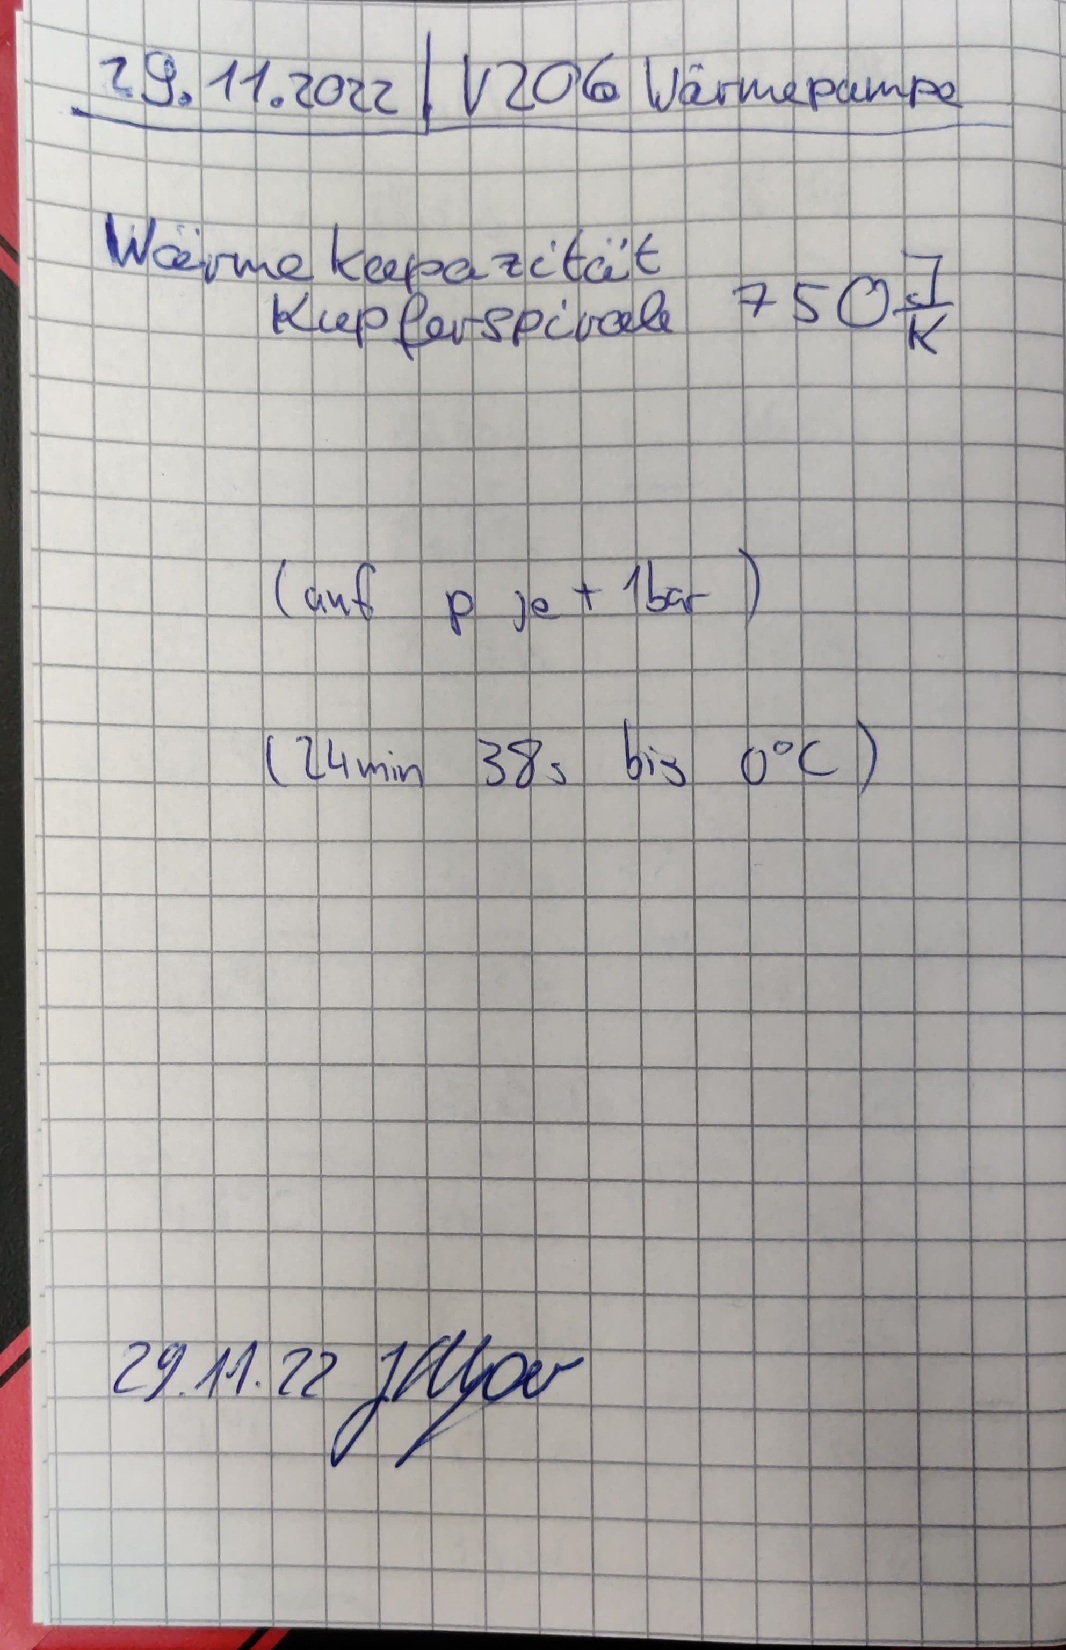
\includegraphics[width=\textwidth, page=1]{v206 Messdaten.pdf}
\end{minipage}
\begin{minipage}[t]{0.45\textwidth}
    \includegraphics[width=\textwidth, keepaspectratio, page=2]{v206 Messdaten.pdf}
\end{minipage}

\begin{minipage}[t]{0.45\textwidth}
    \includegraphics[width=\textwidth, page=3]{v206 Messdaten.pdf}
\end{minipage}

\end{document}